93. $f(x)=\cfrac{x^2+x-6}{2-x}\cdot\sqrt{x^2-2x+1}=\cfrac{(x-2)(x+3)}{2-x}\cdot\sqrt{(x-1)^2}=\begin{cases}-(x+3)|x-1|,\\ x\neq2.\end{cases}=$\\$
\begin{cases}-x^2-2x+3,\ x\in[1;2)\cup(2;+\infty),\\ x^2+2x-3,\ x<1.\end{cases}$
$$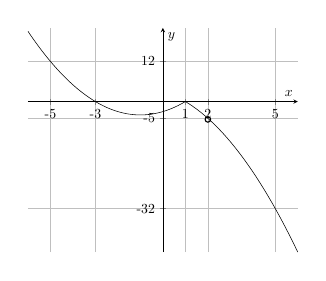
\begin{tikzpicture}[scale=0.5]
\begin{axis}[
    axis lines = middle,
    grid=major,
    legend pos={south west},
    xlabel = {$x$},
    %xlabel style={below right},
    ylabel = {$y$},
    ymin=-45,
    ymax=22,
    xmin=-6,
    xmax=6,
    xtick={-5,-3, 1,2, 5},
    xticklabels={-5,-3, 1,2, 5},
    ytick={-32,-5,12},
    yticklabels={-32,-5,12},
                  ]
	\addplot[domain=1:6, samples=100, color=black] {(-x*x-2*x+3)};
\addplot[domain=-6:1, samples=100, color=black] {(x*x+2*x-3)};
        %\addplot[domain=2.01:6, samples=100, color=black] {2/(2-x)};
   % \addplot[domain=-3:3, samples=100, color=black] {-x};
     %\addlegendentry{$\text{Рис. 1}$};
\end{axis}
\draw (4.57,3.37) circle (2pt);
\end{tikzpicture}$$
